%
% exemplo genérico de uso da classe iiufrgs.cls
% $Id: iiufrgs.tex,v 1.1.1.1 2005/01/18 23:54:42 avila Exp $
%
% This is an example file and is hereby explicitly put in the
% public domain.
%
\documentclass[cic,tc]{iiufrgs}
% um tipo específico de monografia pode ser informado como parâmetro opcional:
%\documentclass[tese]{iiufrgs}
% monografias em inglês devem receber o parâmetro `english':
%\documentclass[diss,english]{iiufrgs}
% a opção `openright' pode ser usada para forçar inícios de capítulos
% em páginas ímpares
% \documentclass[openright]{iiufrgs}
% para gerar uma versão somente-frente, basta utilizar a opção `oneside':
% \documentclass[oneside]{iiufrgs}
\usepackage[utf8]{inputenc}   % pacote para acentuação
\usepackage{times}              % pacote para usar fonte Adobe Times
\usepackage[alf,abnt-emphasize=bf]{abntex2cite}	% pacote para usar citações abnt
\usepackage{graphicx}          % para inserir imagens
\usepackage{booktabs}
\usepackage{float} 
%\usepackage{mathptmx}          % p/ usar fonte Adobe Times nas fórmulas

\graphicspath{ {images/} }

\title{Uma análise dos dados de queimada do INPE no Brasil (preliminar)}
\translatedtitle{Using \LaTeX\ to Prepare Documents at II/UFRGS}

\author{Braz}{José Henrique da Silva}
\advisor[Prof.~Dr.]{Schnorr}{Lucas M.}

% a data deve ser a da defesa; se nao especificada, são gerados
% mes e ano correntes
%\date{maio}{2001}

% o nome do curso pode ser redefinido (ex. para TCs)
\course{Curso de Graduação em Ciência da Computação}

% o local de realização do trabalho pode ser especificado (ex. para TCs)
% com o comando \location:
\location{Porto Alegre}{RS}

% palavras-chave
% iniciar todas com letras maiúsculas
%
\keyword{Formatação eletrônica de documentos}
\keyword{\LaTeX}
\keyword{ABNT}
\keyword{UFRGS}

%
% palavras-chave na lingua estrangeira
% iniciar todas com letras maiúsculas
%
\translatedkeyword{Electronic document preparation}
\translatedkeyword{\LaTeX}
\translatedkeyword{ABNT}
\translatedkeyword{UFRGS}

%
% inicio do documento
%
\begin{document}

% folha de rosto
% às vezes é necessário redefinir algum comando logo antes de produzir
% a folha de rosto:
% \renewcommand{\coordname}{Coordenadora do Curso}
\maketitle

% dedicatoria
\clearpage
\begin{flushright}
\mbox{}\vfill
{\sffamily\itshape
``If I have seen farther than others,\\
it is because I stood on the shoulders of giants.''\\}
--- \textsc{Sir~Isaac Newton}
\end{flushright}

% agradecimentos
\chapter*{Agradecimentos}
Agradeço ao \LaTeX\ por não ter vírus de macro\ldots

% sumario
\tableofcontents

% lista de abreviaturas e siglas
% o parametro deve ser a abreviatura mais longa
% A NBR 14724:2011 estipula que a ordem das abreviações
% na lista deve ser alfabética (como no exemplo abaixo).
\begin{listofabbrv}{SPMD}
	\item[API] Application Programming Interface (Interface de Programação de Aplicação)
	\item[CSV] Comma Separated Values (valores separados por vírgulas).
    \item[GMT] Greenwich Mean Time
    \item[INPE] Instituto Nacional de Pesquisas Espaciais
    \item[IBGE] Instituto Brasileiro de Geografia e Estatística
    \item[URL] Uniform Resource Locator (Localizador Uniforme de Recursos)
    \item[NOAA] National Oceanic and Atmosphere Administration
    \item[MODIS] Moderate Resolution Imaging Spectroradiometer
    \item[GOES] Geostationary Operational Environmental Satellite
    \item[AVHRR] Advanced Very High Resolution Radiometer
\end{listofabbrv}

% idem para a lista de símbolos
%\begin{listofsymbols}{$\alpha\beta\pi\omega$}
%       \item[$\sum{\frac{a}{b}}$] Somatório do produtório
%       \item[$\alpha\beta\pi\omega$] Fator de inconstância do resultado
%\end{listofsymbols}

% lista de figuras
\listoffigures

% lista de tabelas
\listoftables

% resumo na língua do documento
\begin{abstract}
Este documento é um exemplo de como formatar documentos para o
Instituto de Informática da UFRGS usando as classes \LaTeX\
disponibilizadas pelo UTUG\@. Ao mesmo tempo, pode servir de consulta
para comandos mais genéricos. \emph{O texto do resumo não deve
conter mais do que 500 palavras.}
\end{abstract}

% resumo na outra língua
\begin{translatedabstract}
This document is an example on how to prepare documents at II/UFRGS
using the \LaTeX\ classes provided by the UTUG\@. At the same time, it
may serve as a guide for general-purpose commands. \emph{The text in
the abstract should not contain more than 500~words.}
\end{translatedabstract}

% aqui comeca o texto propriamente dito

%%%%%%%%%%%%%%%%%%%%%%%%%%%%%%%%%%%%%%%%%%%%%%%%%%%%%%%%%%%%%%%%%%%%%%%%%%%%%%%

\chapter{Introdução}

O fogo é uma tecnologia que está presente há milênios no território que hoje é o Brasil, desde queimadas controladas pelo povo indígena Kayapó no cerrado para plantio ou caça, até incêndios iniciados por combustão espontânea em períodos de seca no sul da Amazônia. O uso do fogo pelos indígenas era controlado, levando em conta o clima atual e a vegetação a ser queimada, e restrito apenas a um período do ano, com o intuito de reduzir pragas e ajudar nas plantações \citep{leonel_2000}. [P0. O que é uma queimada/fogo] \par

Hoje as queimadas que mais chamam atenção estão diretamente ligadas ao processo de desmatamento e manejo de áreas agrícolas para o cultivo da monocultura de soja. O fogo também é a prática mais barata e rápida para limpar áreas inteiras para a pecuária bovina. Commodites agrícolas e carne bovina movem a economia do Brasil, que é o maior exportador desses produtos, e aumentam a pressão para o desmatamento de novas áreas na Amazônia \citep{fuchs_2020}. [P1. As queimadas hoje] \par

O Brasil ocupa a quarta posição no ranking de nações que mais emitem gases de efeito estufa por habitantes, segundo dados da United Nations Environment Programme (UNEP) de 2022. De acordo com o estudo, o valor absoluto se manteve estável desde 2010, e atingiu seu pico por volta dos anos de 2003 a 2004. Assim como a Indonésia, o que melhor explica a alta posição do Brasil neste ranking são as queimadas e o desmatamento da vegetação nativa. Olhando para os municípios do país, dos dez que mais poluem, oito deles estão localizados no bioma da amazônia e não possuem atividades industriais que justificariam esse valor. [P2. queimadas e efeito estufa no Brasil] \par

\begin{figure}[H]
    \caption{Emissões de gases do efeito estufa per capta de 1990 até 2020 (tCO2e/capita)}
    \begin{center}
        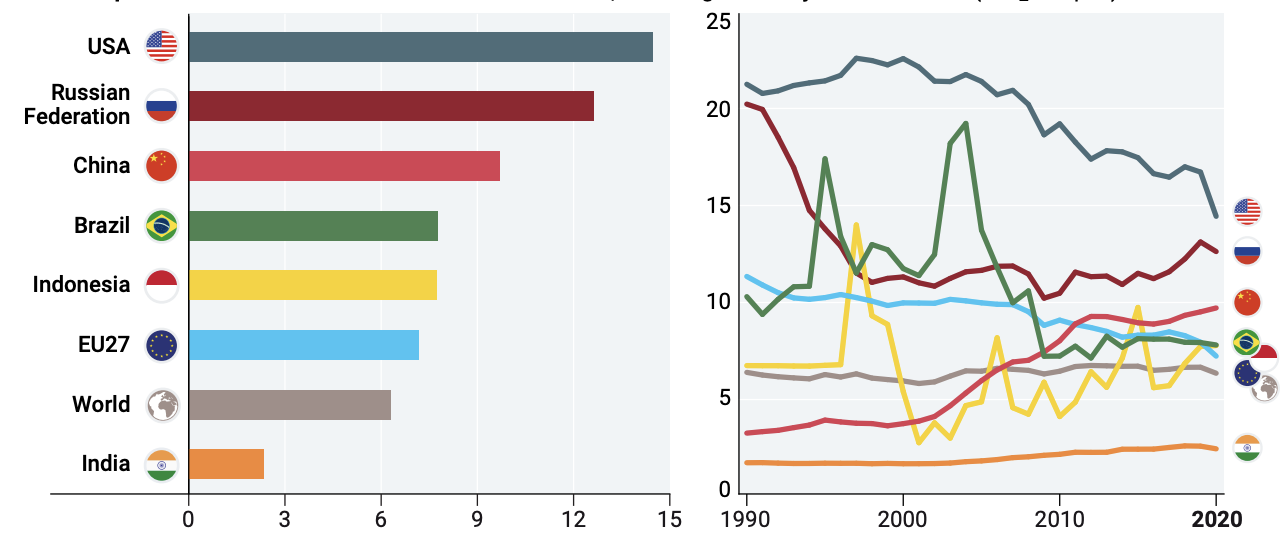
\includegraphics[width=35em]{emissoes_gee_per_capta}
    \end{center}
    \legend{Fonte: Emissions Gap Report 2022: The Closing Window}
    \label{fig:emissoes_gee_per_capta}
\end{figure}

Este trabalho se dedica a estudar e apresentar de forma concisa os dados de focos de queimadas disponibilizados pelo Instituto Nacional de Pesquisas Espaciais (INPE). O principal objetivo é tornar fácil o entendimento desses dados gerados a partir de imagens de satélites, sem a necessidade de um conhecimento prévio das técnicas de ciência de dados e sensoriamento remoto. O escopo de tempo das análises é limitado ao início de 1998, ano que iniciou a base aberta de queimadas, até o final de 2022. [P3. O que é o trabalho em si] \par

Os dados analisados neste trabalho foram obtidos a partir do DBQueimadas, Banco de Dados de Queimadas \url{www.inpe.br/queimadas/bdqueimadas}, que é um sistema desenvolvido pelo INPE e acessível de forma aberta por meio da web. Conta com mais de 300 milhões de pontos coletados desde o ano de 1998, provenientes de vários satélites \citep{setzer2019banco}. Ao disponibilizar os dados das queimadas o instituto possibilita que a sociedade retribua com pesquisas e fomenta novas abordagens ao problema das queimadas no Brasil, como é o caso deste trabalho. [P4. Fonte dos dados usados] \par

Durante o decorrer do documento são apresentadas diversas figuras, a maioria de construção do próprio autor, a fim de instigar a intuição do leitor para o tópico que está sendo abordado. De início, será abordado questões mais teóricas envolvendo caracteríscas dos satélites, suas produções de imagens e como são usadas para detectar um foco ativo de queimada. Após isso, .... [P5. Estrutura do documento] \par

%%%%%%%%%%%%%%%%%%%%%%%%%%%%%%%%%%%%%%%%%%%%%%%%%%%%%%%%%%%%%%%%%%%%%%%%%%%%%%%

\chapter{Conceitos básicos e visão geral dos dados}

Neste capítulo, serão apresentados conceitos importantes para a compreensão do trabalho. Primeiramente, serão formalizadas definições relacionadas às queimadas e à forma como são monitoradas no Brasil. Em seguida, será realizada uma sumarização dos principais satélites utilizados pelo INPE e suas características. Além disso, será abordado como as imagens geradas pelos satélites são utilizadas para a detecção de focos ativos. Por fim, apresentaremos uma análise dos dados para demonstrar uma visão geral das principais tendências e gráficos. \par

\section{O monitoramentos das queimadas no Brasil}

[P0. definir uma queimada, focos detectados e área queimada] \par

[P0. Diferença entre foco detectado e área queimada] \par

[P1. Falar um pouco do INPE e suas divisões] \par

Dentro do site é possível gerar mapas, tabelas, gráficos e exportar os dados sobre as queimadas no Brasil aplicando diferentes filtros. Todo o programa foi desenvolvido com ferramentas abertas, muitas delas criadas pelo próprio time de tecnologia da informação do INPE \citep{setzer2019banco}. [P2. Falamos sobre o programa DBQueimadas] \par

O Banco de Dados de Queimadas é um excelente caso de como os dados abertos podem ajudar a sociedade. Além do DBQueimadas, o INPE também disponibiliza para visualização e download, por meio da Divisão de Geração de Imagens (DGI) \url{www.dgi.inpe.br/catalogo/}, algumas imagens inteiras geradas pelos satélites que o próprio DGI captura e processa. [P3. importancia do dados abertos para a sociedade] \par

Para obter as imagens brutas dos satélites são necessárias antenas especiais que ficam em centros de recepção de dados. Com esse propósito, a DGI possui duas Estações de Recepção e Gravação (ERG) - a primeira em Cachoeira Paulista (SP) e uma mais recente em Cuiabá (MT). Na estação de SP, é feito o processamento de mais de 200 imagens de diversos satélites todos os dias, extraindo os dados de focos ativos de queimadas que alimentam o DBQueimadas. \citep{SiteDGI} [P4. Papel do DGI] \par

É em posse dessas imagens brutas que o INPE aplica algoritmos de detecção de focos de queimadas. No caso da detecção ser positiva, a posição exata (latitude e longitude) e a hora que a imagem foi gerada são adicionadas aos dados como uma nova linha e disponibilizados pelo DBQueimadas. O INPE ainda coloca junto com as coordenadas da detecção mais alguns dados como risco de fogo, poder do fogo, precipitação e dados referentes a região do foco. A lista completa das colunas pode ser vista na Tabela \ref{table:inpeColumns} \cite{PerguntasFrequentesINPE}. [P5. O que é uma observação nos dados] \par

\begin{table}[htbp]
\centering
\caption{Significado de cada coluna dos dados de queimada do INPE}
\begin{tabular}{@{}llp{9cm}@{}}
 \toprule
 \texttt{Atributo} & \texttt{Tipo} & Descrição \\
 \midrule
 \texttt{Id} & \texttt{string} & Identificador único registrado no banco \\
 \texttt{Latitude} & \texttt{double} & Graus decimais da latitude do centro 
                     do pixel de fogo ativo (valores de 90.0000 até -90.0000) \\ 
 \texttt{Longitude} & \texttt{double} & Graus decimais da longitude do centro 
                     do pixel de fogo ativo (valores de 180.0000 até -180.0000) \\  
 \texttt{DataHora} & \texttt{string} & Data a hora da passagem do satélite no fuso 
                     horário de Greenwich (GMT) \\   
 \texttt{Municipio} & \texttt{string} & Nome do município, de acordo com os dados 
                     do IBGE 2000 \\
 \texttt{Estado} & \texttt{string} & Nome do estado \\
 \texttt{Pais} & \texttt{string} & Nome do país \\  
 \texttt{Bioma} & \texttt{string} & Nome do bioma brasileiro, de acordo com 
                     dados do IBGE 2004 (para outros países o campo fica vazio) \\
 \texttt{Precipitação} & \texttt{double} & Valor a precipitação do dia até 
                     o horário da medida (-999 para valores inválidos) \\
 \texttt{DiasSCh} & \texttt{integer} & Dias sem chuva até a data da medida 
                     (-999 para valores inválidos) \\
 \texttt{RiscoFog} & \texttt{double} & Valor do risco de fogo previsto naquele dia 
                     (-999 para valores inválidos) \\
 \texttt{FRP} & \texttt{double} & Fire Radiative Power, MW (megawatts) \\
 \bottomrule
\end{tabular}
\legend{Fonte: O Autor com base em \citet{PerguntasFrequentesINPE}}
\label{table:inpeColumns}
\end{table}

[P7. Como é feito o calculo de área queimada pelo INPE] \par

\section{Os Satélites}

O INPE atualmente processa dados de vários satélites com características distintas entre sí. Estão presentes nos dados desde satélites geoestacionários, como o GOES-12, que está a 29.400 km de distância da superfície \citep{GOES12Algo}, até satélites com óbitas polares, entre 700 a 900 km de altura.[P0. Visao geral dos satelites] \par

Abaixo segue um resumo dos satélites usados pelos INPE desde o início da série histórica até final de 2022 \cite{EmbrapaSatelites}. Os que estão em funcionamento pleno atualmente são: NOAA-20, NOAA-19, NOAA-18, GOES-16, Suomi NPP, AQUA, TERRA, MSG-03, METOP-B e METOP-C. [P1. Falar sobre os principais]\par

\begin{table}[htbp]
\centering
\caption{Características dos satélites usados pelo INPE}
\begin{tabular}{ @{}llllcl@{} }
  \toprule
  Nome    & Sensor & Resolução esp. & Órbita & Lançamento & Passagem \\
  \midrule
  METOP-C & AVHRR-3  & 1100m       & Polar   & 2018 & 21h \\
  NOAA-20 & VIIRS    & 500m        & Polar   & 2017 & 2h / 14h \\
  METOP-B & AVHRR-3  & 1100m       & Polar   & 2012 & 21h \\
  Suomi NPP & VIIRS  & 500m        & Polar   & 2011 & 2h / 14h \\
  NOAA-19 & AVHRR-3  & 1100m       & Polar   & 2009 & 2h / 14h \\
  NOAA-18 & AVHRR-3  & 1100m       & Polar   & 2005 & Variadas \\
  AQUA    & MODIS    & 1000m       & Polar   & 2002 & 2h / 14h \\
  NOAA-17 & AVHRR-3  & 1100m       & Polar   & 2002 & 21h \\
  NOAA-16 & AVHRR-3  & 1100m       & Polar   & 2000 & Variadas \\
  TERRA   & MODIS    & 1000m       & Polar   & 1999 & 11h / 23h \\
  NOAA-15 & AVHRR-3  & 1100m       & Polar   & 1998 & 5h / 17h \\
  TRMM    & VIRS     & 2000m       & Polar   & 1997 & Variadas \\
  NOAA-14 & AVHRR    & 1100m       & Polar   & 1994 & 21h \\
  NOAA-12 & AVHRR    & 1100m       & Polar   & 1991 & 2h / 15h \\
  GOES-16 & ABI      & 2000m       & Geoest. & 2016 & Não se aplica \\
  MSG-03  & SEVIRI   & 3000m       & Geoest. & 2012 & Não se aplica \\
  GOES-13 & GOES I-M & 4000m       & Geoest. & 2006 & Não se aplica \\
  MSG-02  & SEVIRI   & 3000m       & Geoest. & 2005 & Não se aplica \\
  GOES-12 & GOES I-M & 4000m       & Geoest. & 2001 & Não se aplica \\
  GOES-10 & GOES I-M & 4000m       & Geoest. & 1997 & Não se aplica \\
  GOES-08 & GOES I-M & 4000m       & Geoest. & 1994 & Não se aplica \\
  \bottomrule
\end{tabular}
\legend{Fonte: O Autor com base em \citet{EmbrapaSatelites}}
\label{table:satelites}
\end{table}

Cada satélite pode ter um sensor imageador, que gera imagens, com características distintas. Neles são captados imagens não só no comprimento de onda da luz visível (de 400nm a 700nm), mas também no infravermelho (de 780nm a 1mm). Suas medições são divididas em canais, que variam em resolução espacial e espectral (intervalo de comprimento de onda). Geralmente o primeiro canal é dedicado à luz visível, entre o laranja e o vermelho, e com a maior resolução espacial possível para o sensor. Os outros canais utilizam diferentes intervalos do infravermelho e luz visível. [P2. visão geral dos sensores e porque geram dados diferentes] \par

Com todas essas diferenças entre os satélites foi necessário estabelecer um satélite base, que ficou conhecido como Satélite de Referência. Ele é usado para estabelecer uma série temporal e permitir análise de tendência durante vários anos dos focos detectados para diferentes regiões. Este balizador precisa cobrir a área do país de forma satisfatória, ou seja, sua órbita não deve distorcer os dados no geral. Além disso, resoluções dos sensores muito baixas, maiores de 1 km, tornam a análise dos focos pouca precisa. [P3. Satelite de referencia] \par

De 01/junho/1998 a 03/julho/2002 o satélite de referência utilizado foi o NOAA-12 com passagem no final da tarde. Depois desse período passou-se a utilizar o AQUA com passagem à tarde (chamado nos dados de AQUA\_M-T). O satélite AQUA já ultrapassou a data prevista de encerrar o funcionamento em muitos anos e será descontinuado em breve, quando isso acontecer o satélite Suomi NPP será o novo balizador \citep{PerguntasFrequentesINPE}. [P3. Satelite de referencia] \par

Para finalizar, podemos observar na Figura \ref{fig:orbita2022-08-10} a passagem dos satélites no dia 10 de agosto de 2022, gerada a partir de dados do \url{https://celestrak.org/}. Os satélites podem levar vários dias para passar no mesmo local devido a características de sua órbita e podemos ter uma estimativa razoavelmente precisa de sua tragetória ao longo do tempo. Também é possível ver o satélite geoestacioário GOES-16, no norte do perú, representado com um ponto no gráfico. \par

\begin{figure}[H]
    \caption{Órbita dos satélites no dia 10 de agosto de 2022}
    \begin{center}
        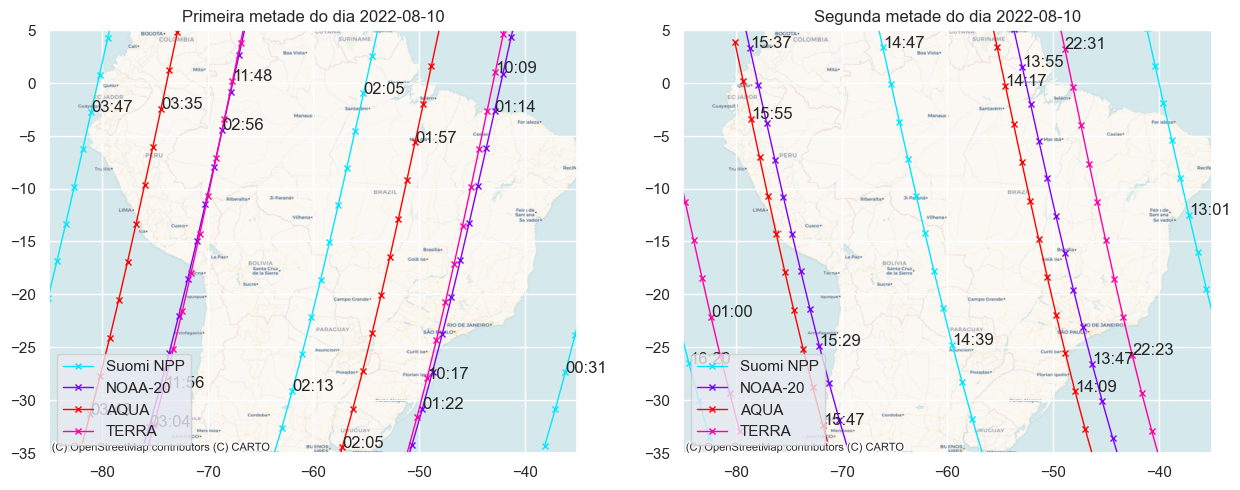
\includegraphics[width=35em]{orbita2022-08-10}
    \end{center}
    \legend{Fonte: O Autor}
    \label{fig:orbita2022-08-10}
\end{figure}

\section{Detecção de focos de queimadas e área queimada}

O algoritmo para identificação de focos ativos é específico para cada tipo de sensor. No geral, eles usam diferentes canais dos sensores dos satélites, entre a luz visível e o infravermelho, e podem ter comportamentos distintos dependendo se a imagem foi gerada à noite ou de dia. Podem também usar limiares dinâmicos, de acordo com a região do planeta, que são calculados com base em uma espécie de média das temperaturas nas regiões próximas ao longo dos dias. Além disso, é comum a aplicação de máscaras para eliminar regiões submersas, costeiras, deserticas e que estavam nubladas na hora da passagem. [P2. Visão geral dos algoritmos para detecçao] \par

Para o caso dos satélites TERRA e AQUA, que têm o sensor MODIS, o instituto mantinha seu próprio método de detecção, que produzia dados de maior confiabilidade \citep{PerguntasFrequentesINPE}. A partir de 2017 o INPE migrou toda a base de dados para o "Collection 6", algoritmo aplicado pela \textit{National Aeronautics and Space Administration} (NASA), marcando o início da chamada Base 2 de queimadas. Anteriormente, a NASA empregava o Collection 5, que gerava falsos positivos em clareiras florestais e falsos negativos para grandes queimadas obscurecidas por fumaça densa.\citep{SCHROEDER2008}. [P3. Algoritmo empregrado pelo INPE] \par

O collection 6 .... \citep{GIGLIO2016} \par

Para detectar áreas queimadas, o instituto atualmente usa o produto AQ1km, desenvolvido em parceria com o Laboratório de Aplicações de Satélites Ambientais (LASA) \citep{SiteAQ1km} que ainda está em fase Provisória (ainda pode sofrer mudanças e não foi validada completamente). O produto é aplicados nos dados do sensor MODIS e, desta forma, usa os satélites AQUA e TERRA de forma concomitante \citep{libonati2015algorithm}. Uma vez que o AQUA foi lançado apenas em 2002, o produto só pode ser usados para dados a partir de 2003. \par

O AQ1km .... \citep{libonati2015algorithm} \par

\section{Uma visão geral dos dados}

Neste subcapítulo, será realizada uma análise inicial dos dados disponíveis sobre focos de queimada, com o objetivo de extrair algumas informações relevantes. É importante, no entanto, ter cuidado na escolha dos satélites a serem utilizados na análise. Para algumas análises, caso sejam usados todos os satélites disponíveis, pode ocorrer a contagem de um mesmo foco várias vezes ou, ainda, a contagem do mesmo foco em passagens diurnas e noturnas de um mesmo satélite polar. Para solucionar esse problema, será utilizado o satélite AQUA com passagem à tarde (AQUA\_M-T), que é  o satélite de referência do INPE atualmente. Dessa forma, é possível evitar a contagem duplicada de focos de queimada e garantir a precisão das informações analisadas. \par

Com relação aos satélites, e possível perceber a partir da Figura \ref{fig:porcentagem_satelites} cinco satélites que mais identificaram focos de queimada em toda a série história, são eles: Suomi NPP, GOES-16, AQUA, NOAA-16 e TERRA. Todos eles estão ativos atualmente e com quantidades de coleta significativas em 2022. AQUA e TERRA são os mais antigos e possuem um sensor obsoleto. O GOES-16 é um satélite geoestacionário, conhecido por gerar dados de forma mais frequente, geralmente detecta apenas queimadas maiores devido a sua posição distante da Terra. Suomi NPP e NOAA-20 possuem um sensor que detecta 10 vezes mais focos que sensor MODIS. Por estar em atividade a mais tempo, o Suomi NPP gerou mais dados que o NOAA-20. \par

\begin{figure}[H]
    \caption{Relação do montante dos dados por satélite}
    \begin{center}
        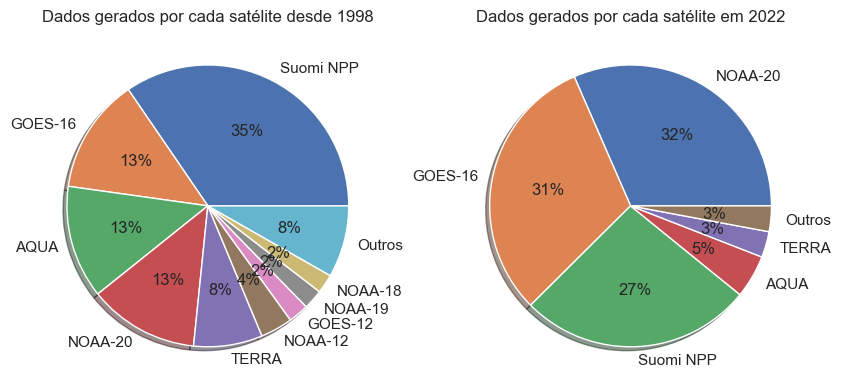
\includegraphics[width=35em]{porcentagem_satelites}
    \end{center}
    \legend{Fonte: O Autor}
    \label{fig:porcentagem_satelites}
\end{figure}

Saber em quais momentos os satélites passam também é importante para a análise. Os satélites polares passam duas vezes por dia no Brasil, variando o local exato da passagem de acordo com as características de sua órbita. Pela Figura \ref{fig:tempo_medidas_satelites} é possível observar esse comportamento empiricamente, em que as 5 primeiras linhas, que representam dados gerados por satélites polares, apresentam dois picos durante um período de 24 horas. Já para o  caso dos geoestacionários (GOES-16), que ficam fixos em relação a uma posição na Terra, não se observou o mesmo padrão. \par

\begin{figure}[H]
    \caption{Amostragem por tempo de cada satélite}
    \begin{center}
        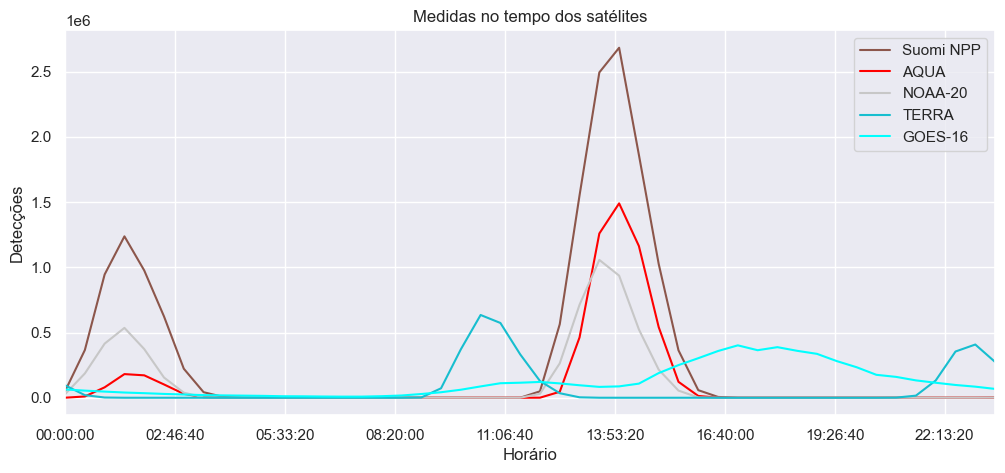
\includegraphics[width=35em]{tempo_medidas_satelites}
    \end{center}
    \legend{Fonte: O Autor, agrupando os dados de queimadas}
    \label{fig:tempo_medidas_satelites}
\end{figure}

A partir de uma análise quantitativa dos dados com relação ao tempo de cada medida, exposto na Figura \ref{fig:quantitativo_geral}, podemos identificar uma grande sazonalidade, sempre tendo picos entre os meses de agosto e setembro. Desde o início da série, o mês que mais teve focos detectados foi setembro de 2007. 

\begin{figure}[H]
    \caption{}
    \begin{center}
        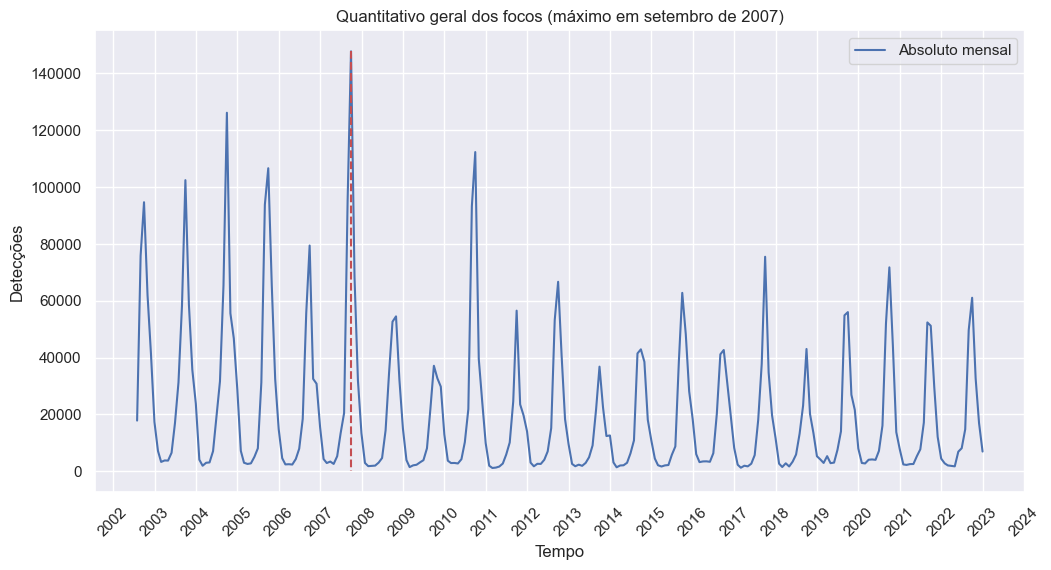
\includegraphics[width=35em]{quantitativo_geral}
    \end{center}
    \legend{Fonte: O Autor, agrupando os dados de queimadas por tempo}
    \label{fig:quantitativo_geral}
\end{figure}


P1. Fazer análise preliminar dos dados gerando alguns gráficos \par
P2. Gráficos geral do brasil com os focos de queimadas totais \cite{geographicDataSciencePython} \par


%%%%%%%%%%%%%%%%%%%%%%%%%%%%%%%%%%%%%%%%%%%%%%%%%%%%%%%%%%%%%%%%%%%%%%%%%%%%%%%

\chapter{Trabalhos Relacionados}

Muitos outros trabalhos antes deste versaram sobre os dados de queimadas do INPE e, em menor escala, especicamente sobre o cálculo das áreas queimadas. Nesse capítulo, serão apresentado alguns trabalhos que estão de alguma forma próximos deste e, no final, será discutido o que faz este de certa forma único. \par

O primeiro estudo refere-se ao trabalho que embasou o produto AQ1km \citep{libonati2015algorithm}, desenvolvido pelo INPE. O objetivo do estudo é detectar áreas queimadas mensalmente por meio de sensoriamento remoto utilizando o sensor MODIS (satélites AQUA e TERRA). Para isso, o algoritmo identifica regiões que apresentaram fogo ativo usando diferentes satélites, extraídos da mesma base do INPE, e agrupa os dados a cada um mês. Em seguida, filtra essas regiões com base em um índice de vegetação sensível a queimadas no espectro do infravermelho próximo, em relação ao mesmo índice do mês anterior. Por fim, identifica regiões próximas às regiões classificadas como área queimada no passo anterior, mas que não apresentaram um indicador forte o suficiente, o que pode ser devido a uma queimada parcial ou baixa intensidade de fogo naquele local. \par



%%%%%%%%%%%%%%%%%%%%%%%%%%%%%%%%%%%%%%%%%%%%%%%%%%%%%%%%%%%%%%%%%%%%%%%%%%%%%%%


\chapter{Metodologia}

Nos primeiros subcapítulos serão abordados as ideias e técnicas gerais da metodologia, sem entrar na implementação desenvolvida. Começa com uma visão geral de como o método é desenvolvido, depois entra em cada pormenor. No final, é discutido como o método foi efetivamente implementado.

\section{Visão geral da metodologia}

A metodologia desenvolvida visa calcular a área de vegetação queimada no Brasil, por meio da análise dos dados de focos de queimadas disponibilizados pelo INPE, juntamente com as características dos diferentes satélites e sensores. A premissa fundamental é que um foco de queimada detectado resulta em uma área queimada. Além disso, considera-se que a quantidade de focos detectados em uma determinada região, em um intervalo de tempo, está diretamente relacionada com a área efetivamente queimada na região. \par 

... apontaram que a detecção de áreas queimadas pode se beneficiar da fusão de observações de incêndios ativos de vários sensores. \citep{giglio2010assessing} ........ mas incendios ativos podem ficar omissos \citep{giglio2009active} ....... \par

.... fazem um diagrama (workflow) .... \par

Para isso, primeiro precisamos entender que o foco detectado por um satélite na verdade representa uma área de abrangência do fogo. Uma vez que estamos em posse das áreas de cada foco detectado de todos os satélites, é possivel proceguir para a próxima fase que é a avaliação das áreas queimadas. Nessa fase, vamos dividir o espaço em pequenos quadrantes e assim avaliá-los separadamente, usando algumas métricas. \par

Para calcular a área queimada dos quadrantes avaliados, é possível utilizar diferentes métodos de avaliação. Um exemplo seria definir um limiar mínimo, acima do qual toda a área do quadrante seria considerada como queimada. Outra possibilidade seria estabelecer uma escala de área do quadrante para que seja considereda como tal. \par

A Figura \ref{fig:exemplo_metodo_completo} ilustra a aplicação completa do método em uma área específica localizada no sudoeste do Pará, durante o dia primeiro ao dia três de setembro de 2022. Na primeira imagem, são mostrados os focos de queimada como pontos, sem nenhum tipo de pré-processamento. Na segunda imagem, os pontos são transformados em áreas. Em seguida, o espaço é divido em quadrantes e avaliados. Na última imagem, é aplicado um cálculo de área queimada levando em conta um limiar de 5 para cada quadrante, resultando em uma área queimada de $33,32 km^2$. \par

\begin{figure}[H]
    \caption{Aplicação do método completo}
    \begin{center}
        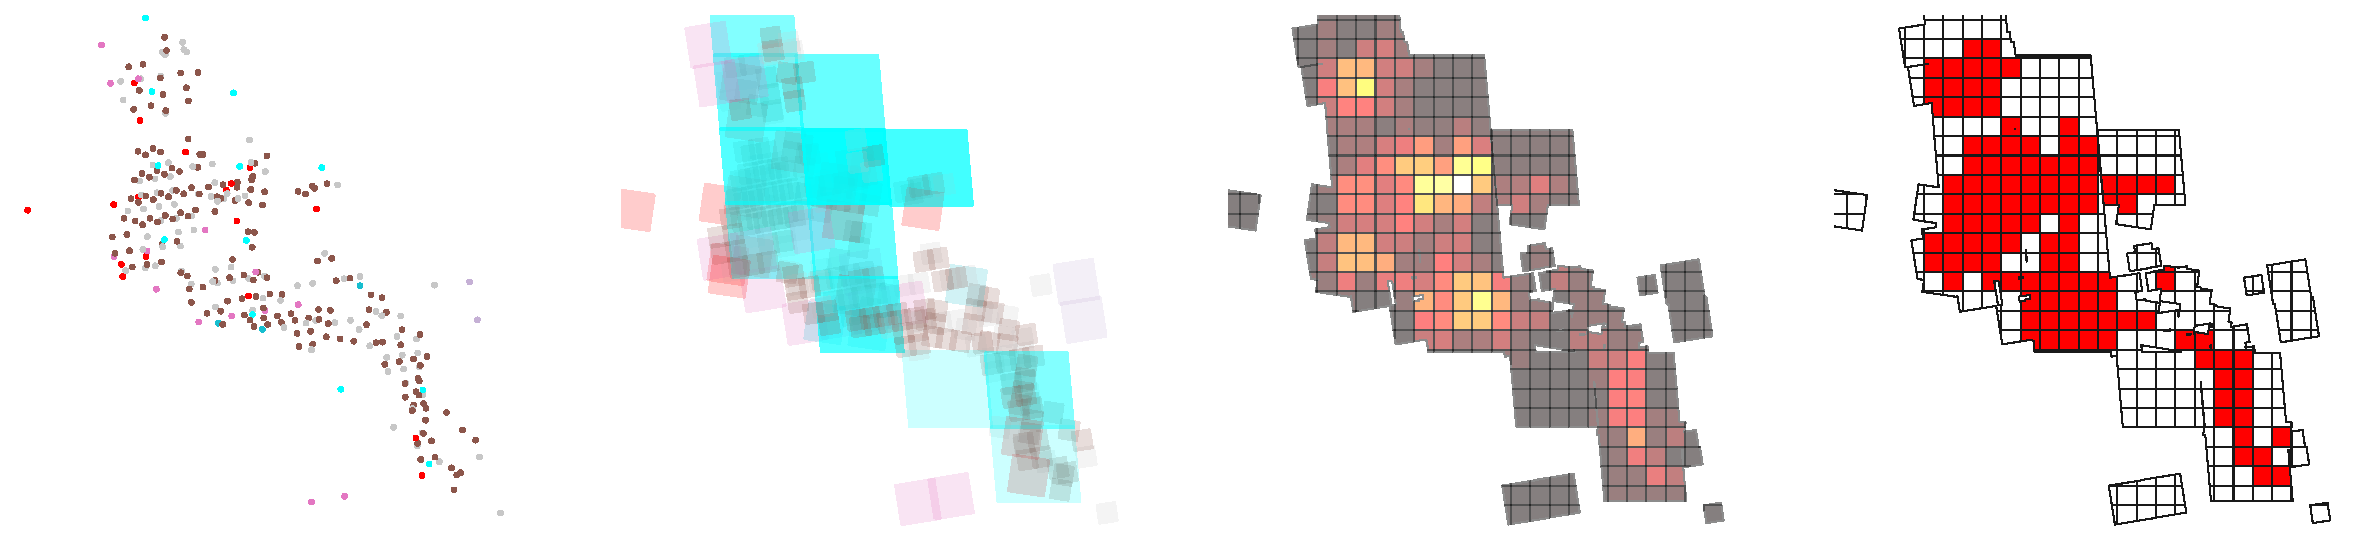
\includegraphics[width=35em]{exemplo_metodo_completo}
    \end{center}
    \legend{Fonte: O Autor, aplicando o método}
    \label{fig:exemplo_metodo_completo}
\end{figure}

\section{Área abrangida por uma medição}

Quando um foco de queimada é detectado por algum satélite, ele representa uma área quadrada aproximadamente do tamanho da resolução de seu sensor. Ou seja, um foco dectado por um satélite AQUA, que utiliza o sensor MODIS, representa uma área de $\approx1Km^2$. Para um satélite com o sensor menos preciso, como o GOES-13, que utiliza o sensor GOES I-M com resolução espacial de $4Km$, a área representada seria 16 vezes maior, indicando uma menor precisão. [Visão geral aproximada] \par

O cálculo exato da área coberta pela medição deve levar em conta as distorções ocorridas pela diferença de localização entre o ponto da medição ($p_m$) e a localização  do satélite ($p_s$). Quanto maior a distância entre os dois pontos, maior será a distorção em relação a área de corbertura do sensor. Para um satélite geoestácionário, por exemplo, essa distância é sempre muito grande, devido a sua órbita com altura em torno do $35Km$. \par

Outro fator que afeta a área coberta é a inclinação dos satélites. Os satélites que orbitam a Terra em órbitas polares, possuem uma determinada inclinação que lhes permitem cobrir diferentes áreas de todo o planeta durante sua tragetória (Figura \ref{fig:orbita2022-08-10}). Quando o satélite está se movendo em uma trajetória ascendente, ou seja, do sul para o norte, a área coberta pelo sensor deve ser rotacionada com um fator positivo. Por outro lado, se a trajetória for descendente, do norte para o sul, o fator de rotação será negativo. \par

A Figura \ref{fig:comparacao_pontos_e_areas} apresenta dados coletados pelo satélite  Suomi NPP no dia dois de setembro de 2022. O primeiro par de imagens corresponde à órbita ascendente do satélite, enquanto o segundo par de imagens corresponde à órbita descendente. Observa-se que, na primeira e terceira imagens, os pontos dos focos de queimada estão alinhados, mas ligeiramente rotacionados em alguns graus, coincidindo com a inclinação do satélite. Na segunda e quarta imagens, os pontos ganham a área do sensor ($500m$) e encaixam perfeitamente entre seus vizinhos. \par

\begin{figure}[H]
    \caption{Comparação entre pontos e áreas dos focos detectados pelo satélite Suomi NPP}
    \begin{center}
        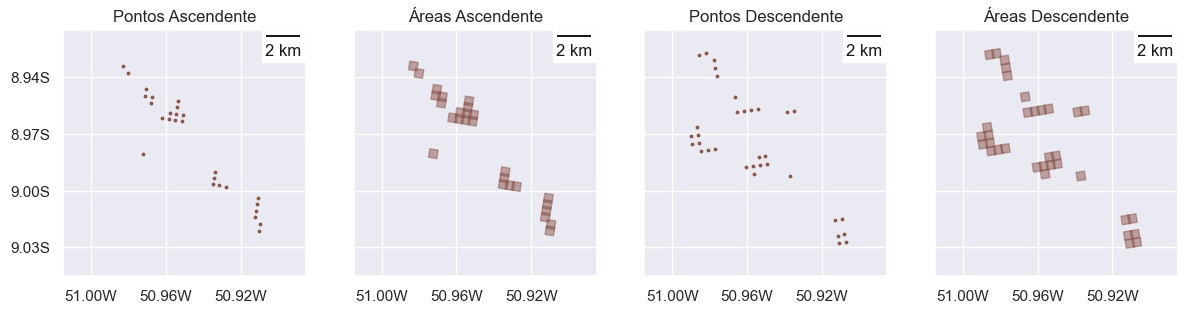
\includegraphics[width=35em]{comparacao_pontos_e_areas}
    \end{center}
    \legend{Fonte: O Autor, aplicando o método de cálculo de áreas}
    \label{fig:comparacao_pontos_e_areas}
\end{figure}

\section{Separação e quantificação de quadrantes}

A separação entre quadrantes é a forma de discretizar os dados do espaço, que são continuos. Os quadrantes abstraem os detalhes das medições dos diferentes satélites, com diferentes áreas e orientações. Como resultado, temos um gride regular que é usado para as operações de avaliação de serão descritas a seguir. \par

A separação em quadrantes também foi planejada para melhorar o desempenho do processamento. Ao dividir o problema em partes menores, é possível resolver cada uma de forma paralela, pois as avaliações dos quadrantes são independentes entre si. Além disso, com a utilização de índices espaciais, usados nos cálculos de intersecção, o processamento dos quadrantes é ainda mais otimizado. Quanto maior o quadrante usado, menos avaliações são necessárias, porém a precisão da área queimada também diminui. Como se trata de um espaço bidimensional, a complexidade computacional da avaliação em relação à quantidade de quadrantes é $O(n^2)$. \par

Com base em experimentos, foi constatado que o uso de quadrantes muito pequenos (com menos de 0,002 graus quadrados) não aumentam significativamente a precisão dos resultados e tornam a execução muito mais demorada. Portanto, o valor recomendado para o tamanho dos quadrantes fica em torno de 0,004 a 0,005 graus, o que coincide com o tamanho da menor resolução de sensor presente nos dados, que é o VIIRS de 500m. A Figura \ref{fig:diferenca_entre_quadrantes} ilustra como a mudança no tamanho do quadrante impacta na quantidade deles e na sua avaliação. \par

\begin{figure}[H]
    \caption{Diferença da avaliação para diferentes tamanhos de quadrantes}
    \begin{center}
        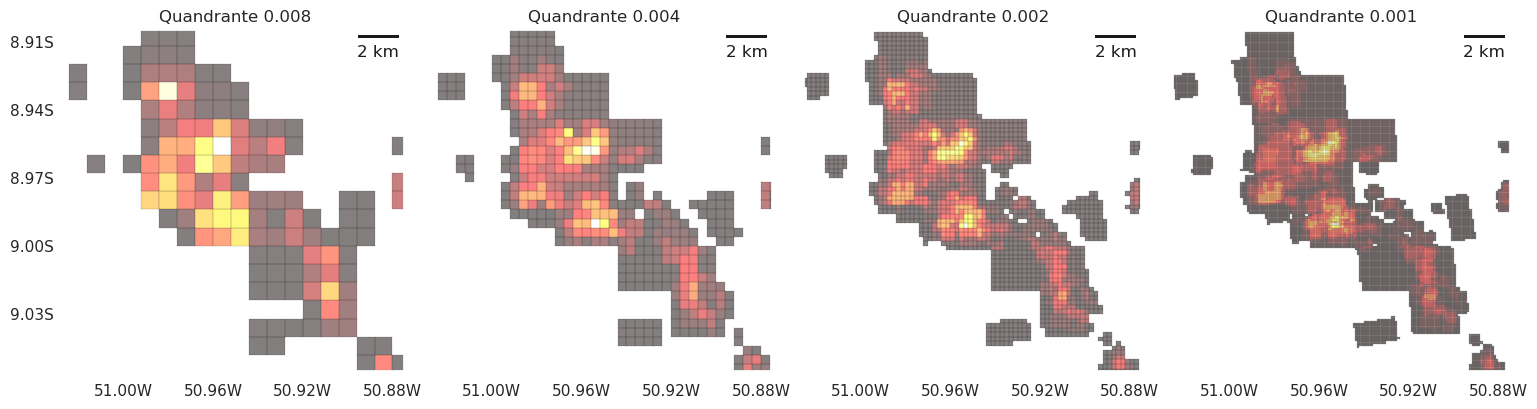
\includegraphics[width=35em]{diferenca_entre_quadrantes}
    \end{center}
    \legend{Fonte: O Autor, variando o tamanho dos quadrantes em uma mesma área}
    \label{fig:diferenca_entre_quadrantes}
\end{figure}

Com a distribuição dos quadrantes definida, é necessário atribuir a cada um deles um valor que represente a probabilidade de que a área contida tenha sido queimada. Sendo $q$ o quadrante a ser avaliado; $M$ um conjunto de todas as medições; operação $area(p)$ retorna a área de um polígono $p$; operação $unique\_satelite(Q)$ retorna todos os satélites diferentes do conjunto $Q$; $min\_area$ é a área mínima; A definição formal da avaliação é dada por: \par

\begin{equation} \label{eqn:def_qm}
Qm = \{ m \in M \mid m \cap q \}
\end{equation}

\begin{equation} \label{eqn:def_qm_line}
Qm' = \{ m \in Qm \mid area\left(m\right) \ge min\_area \}
\end{equation}

\begin{equation} \label{eqn:def_us}
Us = \{ m \in unique\_satelite\left(Qm'\right) \}
\end{equation}

\begin{equation} \label{eqn:def_ia}
ia = \left(\sum_{m}^{Qm'} area\left(m\right)\right) \div area(q)
\end{equation}

\begin{equation} \label{eqn:def_aq}
aq = |Us|^2 + min\left(ia, 3.99\ldots \right)
\end{equation}

Para cada quadrante ($q$), é realizado o cálculo da intersecção com cada medição ($m$) contida nele, resultando em um conjunto $Qm$ (\ref{eqn:def_qm}). Em seguida, é realizada uma filtragem no conjunto $Qm$, removendo todos os elementos que não possuem uma determinada área mínima (por padrão definido como 20\% da área total do quadrante $q$), resultando em $Qm'$ (\ref{eqn:def_qm_line}). A partir de $Qm'$, é extraído o número de satélites diferentes presentes nesse conjunto, que é denominado $Us$ (\ref{eqn:def_us}). Além disso, é calculada a soma das áreas de $Qm'$ e dividida pela área total de $q$, resultando em $ia$ (\ref{eqn:def_ia}). Finalmente, a avaliação final do quadrante ($aq$) é obtida pela expressão \ref{eqn:def_aq}. \par

De forma mais alto nível, a avaliação dos quadrantes valoriza significativamente aqueles que apresentam medições de diferentes satélites. Essa abordagem justifica-se pelo fato de que ajuda a reduzir os ruídos nas medições e a identificar queimadas mais intensas. Além disso, diferentes satélites realizam medições em horários distintos (veja a Figura \ref{fig:tempo_medidas_satelites}), o que indica uma queimada mais prolongada. Em ambos os casos, queimadas mais intensas e duradouras sinalizam um maior potencial de o fogo se espalhar para outras áreas da vegetação. \par

A segunda parte da avaliação visa evitar que medições muito pequenas tenham um impacto significativo no resultado final do quadrante, mesmo que hajam muitas delas. 
Para isso, basicamente calcula quantas vezes a área das medições somadas cabem no quadrante. Ou seja, são medições que estão no quadrante mas que tem pouca probabilidade de indicar uma queimada naquele quadrante específico. Além disso, é importante destacar que quadrantes com medições de apenas um satélite têm um valor limitado de $4.99\ldots$ ($1^2 + 3.99\ldots$). Essa limitação serve como uma penalização para os quadrantes que possuem pouca diversidade de dados, incentivando a valorização de quadrantes com medições de diferentes satélites e, portanto, uma maior probabilidade da área ter sido queimada. \par

\section{Cálculo da área queimada}

Finalmente, com os quadrantes avaliados, é possível estimar a área queimada para cada quadrante. É importante que o método de cálculo seja flexível, permitindo que o pesquisador teste diferentes métodos ou treine um modelo de aprendizado de máquina. Uma forma de fazer isso é atribuir um número que represente a porcentagem de área queimada dentro do quadrante e, em seguida, multiplicá-lo pela área total do quadrante para obter a área queimada dentro do quadrante. Após calcular a área queimada de cada quadrante, é necessário somar todos esses valores para obter a área total queimada. \par

Nesse sentido, o papel do pesquisador é definir uma função ($eval(v)$) que receba o valor do quadrante, calculado no passo anterior, e retorne um número real entre zero e um. Essa função também pode receber o maior e o menor valor presente na avaliação dos quadrantes, que podem ser usados para normalizar as áreas. \par

Para facilitar o trabalho do pesquisador, a implementação pode fornecer funções built-in comuns que definem a função $eval(v)$. Na Figura \ref{fig:eval_func_built_in}, são apresentadas algumas possibilidades de definições para essa função. A função mais simples é chamada de limiar, que estabelece que toda a área do quadrante deve ser considerada queimada se a avaliação for maior que um determinado valor e nenhuma área deve ser considerada queimada se não alcançar esse valor. Outra função simples é a linear, que faz o valor da área queimada crescer de forma linear dentro de um valor máximo e mínimo. A última função é a exponencial, semelhante à linear, mas com uma exponenciação que faz o valor crescer mais lentamente no início e de forma mais acentuada no final do intervalo. \par

\begin{figure}[H]
    \caption{Funções built-in para cálculo de área}
    \begin{center}
        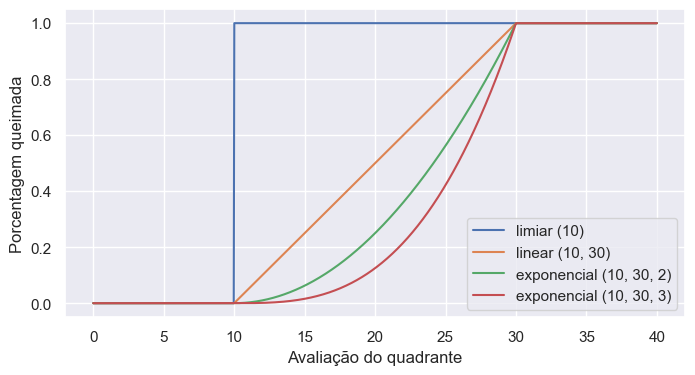
\includegraphics[width=25em]{eval_func_built_in}
    \end{center}
    \legend{Fonte: O Autor}
    \label{fig:eval_func_built_in}
\end{figure}

A Figura \ref{fig:aplicacao_funcoes_built_in} mostra como as diferentes funções e parâmetros podem gerar resultados bem diferentes. .... \par

\begin{figure}[H]
    \caption{Exemplo da aplicação das funções built-in}
    \begin{center}
        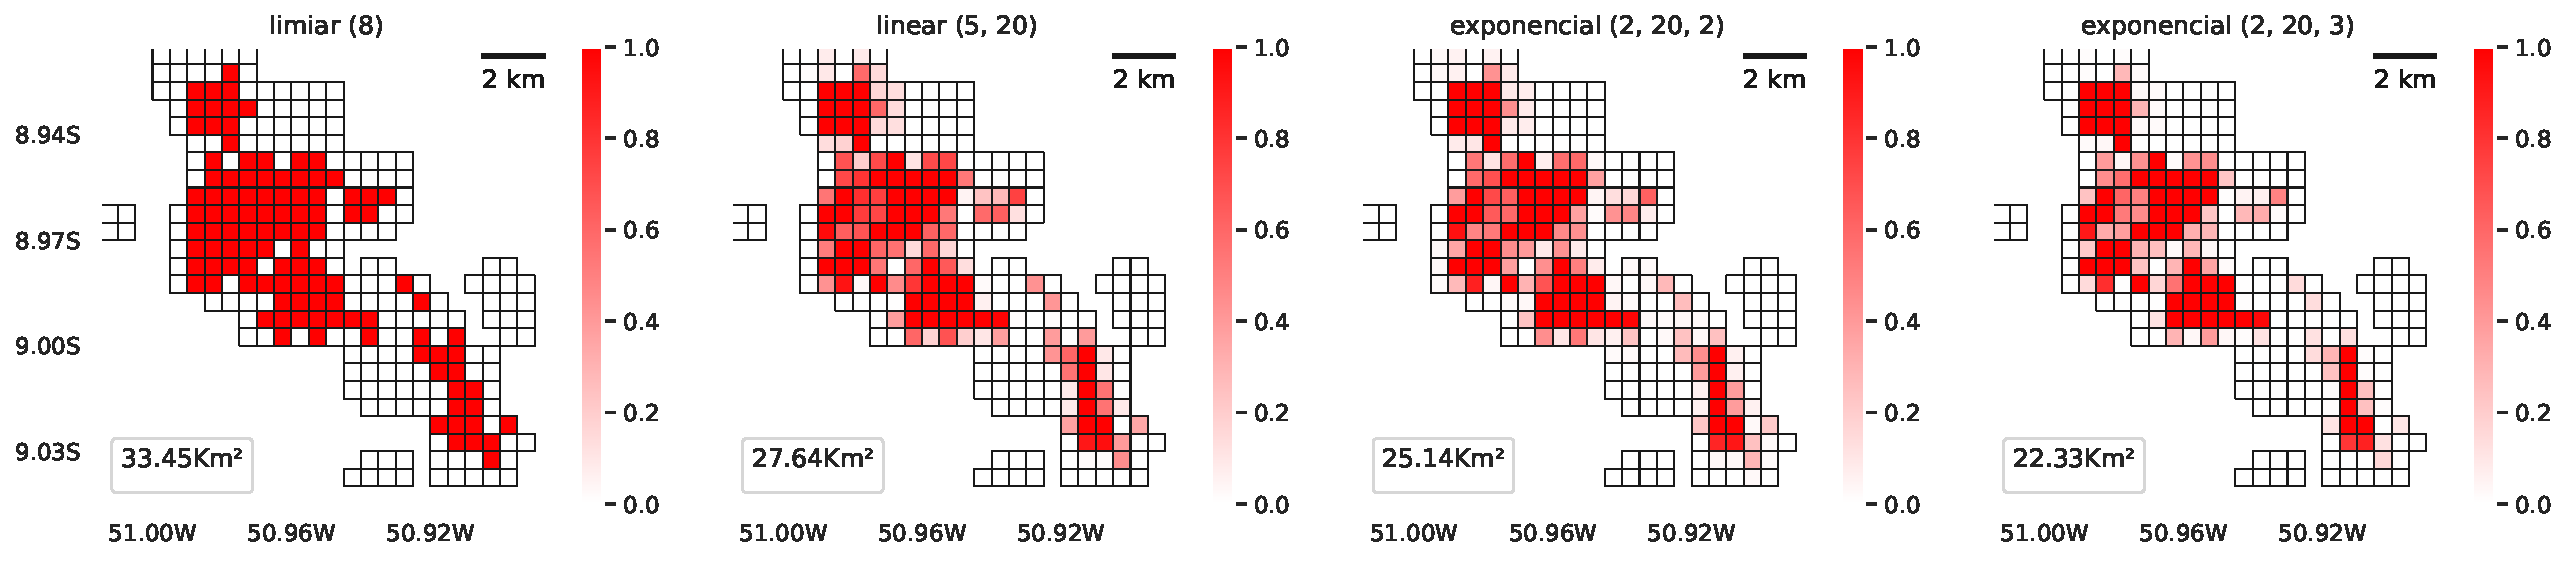
\includegraphics[width=35em]{aplicacao_funcoes_built_in}
    \end{center}
    \legend{Fonte: O Autor}
    \label{fig:aplicacao_funcoes_built_in}
\end{figure}


%% Aqui começa a implementação
\section{Coleta dos dados}

Uma parte importante do processo foi coletar os dados do site DBQueimadas. Para exportar os dados utilizando o navegador de internet, é necessário preencher um formulário os campos de data inicial,data final e um endereço de e-mail. O intervalo de tempo não pode exceder um ano. Também é possível aplicar filtros ainda mais detalhados como: continente, país, estado, município, satélite, bioma e unidades de conservação/terras indígenas. Após clicar em "Exportar", uma mensagem é enviada para o e-mail informado no formulário contendo link de download dos dados requisitados. O arquivo disponibilizado é um CSV compactado como um zip. \par

Apesar de ser um site com boas métrica e usabilidades, seria praticamente inviável baixar todos os dados do Brasil de forma manual. Nesse sentido, foi necessário entender quais eventos são disparados quando solicitamos os dados pelo site a fim de automatizar o processo de download. \par

Foi identificado que na verdade o site faz uma requisição GET para a API do DBQueimadas, localizada em \url{https://queimadas.dgi.inpe.br/queimadas/exportacaobdq/exportar}, passando nos parâmetros da URL os filtros informados pelo usuário, codificados em JSON. Além dos filtros, também é necessário informar o e-mail e o formato de arquivo desejado. Um exemplo de uso dessa API, por meio de uma invocação CURL, pode ser encontrado no \ref{anexo:usoApiInpe} \par

A fim de automatizar o processo, foi desenvolvido um script em Python que solicita os dados referentes a 30 dias, totalizando 300 requisições de 1998 até 2022. Com o intuito de não sobrecarregar os servidores do INPE, foi adicionada uma espera de um minuto a cada requisição. \par

Para o processo ser concluído, ainda seria necessário fazer o download do arquivo por meio do link enviado por e-mail. Lançou-se mão do Google Scripts, uma ferramenta que possibilita escrever programas simples, em uma liguagem parecida com JavaScript, e tem integração com os serviços do Google (como o Gmail). A partir dessa ferramenta foi possível extrair o link de cada mensagem e finalmente salvar o arquivo de forma automatizada. \par

Todos esse processo de investigação e recuperação dos dados levou cerca de uma semana. Todos os arquivos baixados ocupam pouco mais de 4 Gigabytes de armazenamento em disco e somados tem exatamente 43.782.758 linhas. Ao final, eles foram recompactados em um único zip (450 Megabytes) e estão disponíveis em \url{https://bit.ly/3IgHIXH} para download de forma independete aos servidores do INPE. \par

Também lançou-se mão dos dados públicos territoriais do Instituto Brasileiro de Geografia e Estatística (IBGE) com o intuito de gerar gráficos delimitados em municípios, unidades federativas e biomas. Todos os arquivos baixados estão em formato Shapefile, responsável por armazenar dados vetoriais geográficos. \par

\section{Implementação do método}

Para análise dos dados, foram utilizadas diversas ferramentas do ecossistema Python para Data Science, tais como NumPy, Pandas e Matplotlib. Além disso, foram empregadas bibliotecas específicas para análise de dados geográficos, como GeoPandas, Pysal, Xarray e Shapely. Para garantir a reprodutibilidade das execuções e a organização do código, foi adotado o Jupyter Notebook. Todos os artefatos gerados durante o projeto podem ser encontrados em \url{https://github.com/josebraz/INPE-Queimadas}, disponibilizados sob a licença MIT. \par

A biblioteca GeoPandas é uma extensão do Pandas, adicionando uma coluna especial chamada 'geometry'. Essa coluna define as coordenadas e o formato dos dados em um sistema de coordenadas predefinido. O GeoPandas também integra-se com a biblioteca Shapely, que é usada para cálculos de estruturas geométricas espaciais. Com essa biblioteca, é possível realizar operações da teoria dos conjuntos em elementos geométricos, como união, interseção e diferença, entre outras. \par

[falar sobre suporte a Spatial index https://autogis-site.readthedocs.io/en/2019/notebooks/L3/spatial-join.html] \par

\section{Pre processamento (ignorar)}
%%%%%%%%%% Carregando os dados para análise e pre processamento

Os 300 arquivos das queimadas foram carregados para o Pandas e depois concatenados
em uma única estrutura de DataFrame. Houve a necessidade de converter o timezone 
das datas (que eram em UTC) para o timezone de Brasília, a fim de gerar gráficos 
de mais fácil entendimento para brasileiros. As colunas de texto foram convertidas 
para categorias, espécies de enumerações no Pandas, reduzindo o espaço ocupado 
de memória, uma vez que muitos valores acabavam se repetindo na mesma coluna. 
[P1. pre processamentos dos dados]\par

Como parte do pré-processamento dos dados, foi identificado regras de nomenclaturas 
especiais para alguns satélites. Para o AQUA (AQUA\_M-T e AQUA\_M-M) e TERRA 
(TERRA\_M-T e TERRA\_M-M), a primeira letra M representa o sensor MODIS e a última
letra indica em que período do dia foi a passagem do satélite, sendo M para Manhã 
e T para Tarde. Outros satélites como Suomi NPP, NOAA-19, NOAA-18, NOAA-16, NOAA-15 
e NOAA-12 também podem apresentar a última letra do nome sendo D para Diurno.
A partir do entendimento dessa regra de nomenclatura, foi possível criar uma nova 
coluna que informa o nome simplificado dos satélites, a fim de facilitar 
algumas análises. Em comparação com a coluna original dos satélites, que tinha 32 
valores possíveis, a nova coluna contém apenas 22 valores possíveis.
[P2. Explicar equivalencias entre os satelites] \par

A partir da coluna de nomes de satélites simplificada foi possível atribuir cores 
únicas para cada um (Figura \ref{fig:cores_satelites}), de forma a padronizar os 
gráficos e facilitar o entendimento.

\begin{figure}[H]
    \caption{Cores escolhidas para cada satélite}
    \begin{center}
        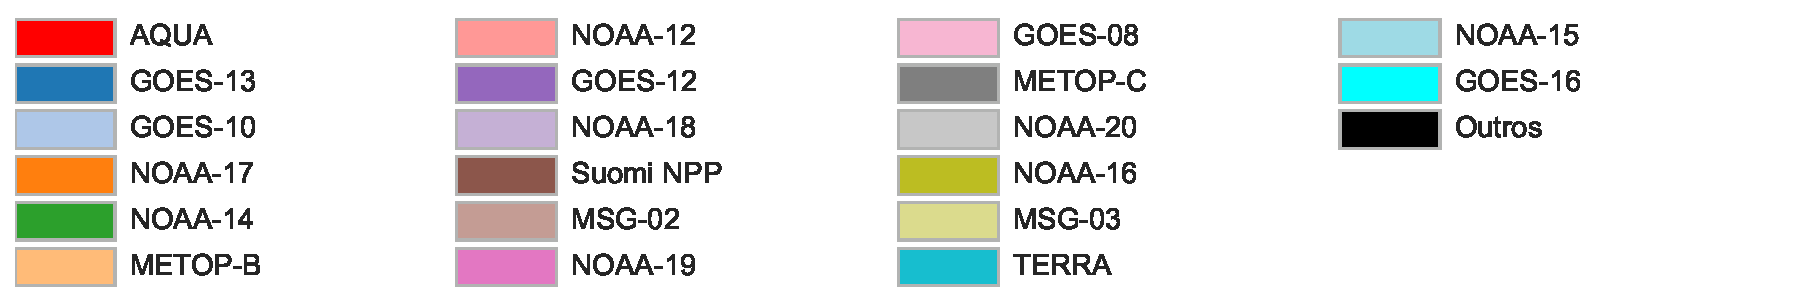
\includegraphics[width=35em]{cores_satelites}
    \end{center}
    \legend{Fonte: O Autor}
    \label{fig:cores_satelites}
\end{figure}



%%%%%%%%%%%%%%%%%%%%%%%%%%%%%%%%%%%%%%%%%%%%%%%%%%%%%%%%%%%%%%%%%%%%%%%%%%%%%%%

\chapter{Resultados e Discussão}


%%%%%%%%%%%%%%%%%%%%%%%%%%%%%%%%%%%%%%%%%%%%%%%%%%%%%%%%%%%%%%%%%%%%%%%%%%%%%%%

\chapter{Considerações Finais}

%%%%%%%%%%%%%%%%%%%%%%%%%%%%%%%%%%%%%%%%%%%%%%%%%%%%%%%%%%%%%%%%%%%%%%%%%%%%%%%


\bibliographystyle{abntex2-alf}
\bibliography{biblio}

\end{document}
